\documentclass[tikz,border=3pt]{standalone}
\usepackage[utf8]{inputenc}
\usepackage[T1]{fontenc}
\usepackage{lmodern}
\renewcommand{\familydefault}{\sfdefault}
\usepackage{sansmath}\sansmath
\usepackage{chemfig}
\usepackage{pgfplots}\pgfplotsset{compat=1.18,/pgf/number format/use comma,/pgf/number format/1000 sep={.}}
\usetikzlibrary{arrows.meta,calc,positioning,decorations.pathmorphing,patterns}
% paleta del sitio
\definecolor{nar}{HTML}{E8680C}\definecolor{narc}{HTML}{FFB35C}\definecolor{hielo}{HTML}{FFF3E8}
\definecolor{tinta}{HTML}{1D1D1F}\definecolor{gris}{HTML}{6E6E73}\definecolor{lila}{HTML}{7C5CF0}
\definecolor{azul}{HTML}{2F6FD6}\definecolor{menta}{HTML}{17A673}\definecolor{coral}{HTML}{E8342A}
\begin{document}
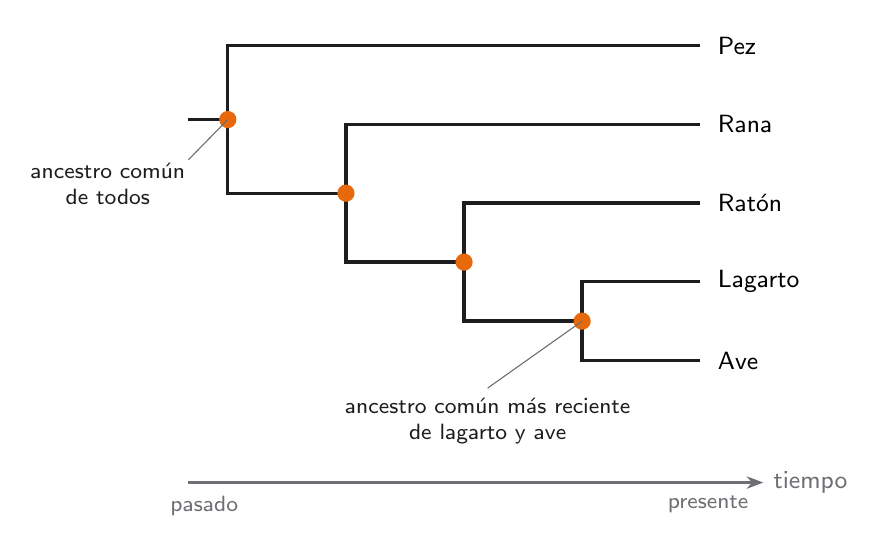
\begin{tikzpicture}[font=\small,rama/.style={tinta,very thick},nodo/.style={circle,fill=nar,inner sep=2.2pt}]
% puntas: Pez 4, Rana 3, Raton 2, Lagarto 1, Ave 0
\draw[rama] (0,3.06) |- (6,4);
\draw[rama] (0,3.06) |- (1.5,2.125);
\draw[rama] (1.5,2.125) |- (6,3);
\draw[rama] (1.5,2.125) |- (3,1.25);
\draw[rama] (3,1.25) |- (6,2);
\draw[rama] (3,1.25) |- (4.5,0.5);
\draw[rama] (4.5,0.5) |- (6,1);
\draw[rama] (4.5,0.5) |- (6,0);
\draw[rama] (-0.5,3.06) -- (0,3.06);
\foreach \p in {(0,3.06),(1.5,2.125),(3,1.25),(4.5,0.5)} \node[nodo] at \p {};
\foreach \n/\y in {Pez/4,Rana/3,Ratón/2,Lagarto/1,Ave/0} \node[anchor=west] at (6.1,\y) {\n};
\draw[gris,thin] (4.5,0.5) -- (3.3,-0.35) node[anchor=north,text=tinta,align=center,font=\footnotesize] {ancestro común más reciente\\de lagarto y ave};
\draw[gris,thin] (0,3.06) -- (-0.5,2.55) node[anchor=north east,inner sep=1pt,text=tinta,align=center,font=\footnotesize] {ancestro común\\de todos};
\draw[-{Stealth[length=6pt]},gris,thick] (-0.5,-1.55) -- (6.8,-1.55) node[anchor=west,text=gris] {tiempo};
\node[text=gris,font=\footnotesize,anchor=north] at (-0.3,-1.6) {pasado};
\node[text=gris,font=\footnotesize,anchor=north] at (6.1,-1.6) {presente};
\end{tikzpicture}
\end{document}
